\subsection{Code Examples}
Figure \ref{fig:javaClassesTempl} shows the coding style we used for
classes in Java. As explained the curly braces are beneath the class
declarations and method, variables are in lower camel case, while
constants are all upper case and constructors are upper camel case. 

Figure \ref{fig:javaInterfacesTempl} shows the coding style for a 
Java interface. As explained the names of interfaces are prepended
with a capital \emph{I}.

\begin{figure}[h]
	\begin{center}
		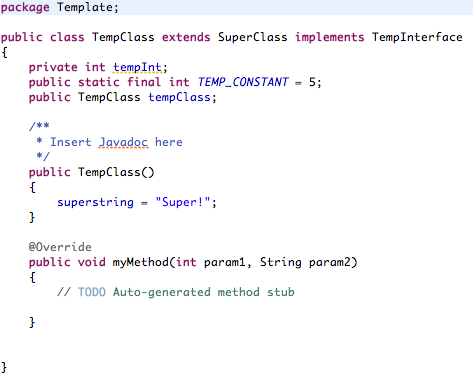
\includegraphics[width=12cm]{Pictures/CodeTemplate1}
	\end{center}
	\caption{Java Classes}
	\label{fig:javaClassesTempl}
\end{figure}

\begin{figure}[h]
	\begin{center}
		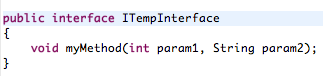
\includegraphics[width=8cm]{Pictures/CodeTemplate2}
	\end{center}
	\caption{Java Interfaces}
	\label{fig:javaInterfacesTempl}
\end{figure}